% !TeX root = ../main.tex

\section{Initialization Study}
\label{sec:abs1-init}

\subsection*{Experimental Variants}
We test five weight-initialization schemes—\textsc{tiny}, \textsc{normal},
\textsc{Xavier}, \textsc{Kaiming}, and \textsc{large}—were evaluated under
identical training conditions (Adam, $lr=0.01$, $50$ seeds, early-stop at
$\mathcal L<10^{-7}$).  The following subsections present classification
accuracy, convergence timing, weight-space movement, and geometric outcomes.

% ------------------------------------------------------------------
\subsection*{Classification Accuracy}

\begin{table}[h]
\centering
\caption{Number of runs (out of 50) achieving each discrete accuracy level
on the centred XOR dataset.  All variants ultimately attain $100\,\%$
accuracy.}
\label{tab:abs1-init-accuracy}
\begin{tabular}{lccccc}
\toprule
\multirow{2}{*}{Init} & \multicolumn{5}{c}{Accuracy level}\\
\cmidrule(lr){2-6}
 & 0\% & 25\% & 50\% & 75\% & 100\% \\
\midrule
Tiny    & 0 & 0 & 0 & 0 & 50 \\
Normal  & 0 & 0 & 0 & 0 & 50 \\
Xavier  & 0 & 0 & 0 & 0 & 50 \\
Kaiming & 0 & 0 & 0 & 0 & 50 \\
Large   & 0 & 0 & 0 & 0 & 50 \\
\bottomrule
\end{tabular}
\end{table}

\textbf{Discussion.}  
Because the analytic optimum is reachable from any orientation, every
initializer eventually yields perfect XOR classification.  The accuracy table
will become more informative in later chapters where deeper models can stall
at intermediate performance plateaus.

% ------------------------------------------------------------------
\subsection*{Convergence Timing}

\begin{table}[h]
\centering
\caption{Epochs to reach $\mathcal L<10^{-7}$ (percentiles over 50 runs).}
\label{tab:abs1-init-epochs}
\begin{tabular}{lccccc}
\toprule
Init & 0\,\% & 25\,\% & 50\,\% & 75\,\% & 100\,\% \\
\midrule
Tiny    & 75  & 141 & 147 & 154 & 166 \\
Normal  & 76  & 127 & 146 & 164 & 297 \\
Xavier  & 62  & 122 & 151 & 234 & 449 \\
Kaiming & 61  & 139 & 198 & 266 & 548 \\
Large   & 154 & 527 & 671 & 878 & 1670 \\
\bottomrule
\end{tabular}
\end{table}

\textbf{Discussion.}  
Convergence time grows monotonically with initial weight scale.  Tiny and
Normal inits start close to the optimal norm and need mainly a small rotation,
whereas Large must shrink by orders of magnitude before fine-tuning—the
principal driver of its median $671$-epoch runtime.

% ------------------------------------------------------------------
\subsection*{Weight Orientation and Scale}

\begin{table}[h]
\centering
\caption{Median angle (°) between initial and final weights and median
norm ratio $\lVert W_{\text{init}}\rVert / \lVert W_{\text{final}}\rVert$.}
\label{tab:abs1-init-angle-norm}
\begin{tabular}{lcc}
\toprule
Init & Angle (median) & Norm ratio (median) \\
\midrule
Tiny    & 22.0 & 0.16 \\
Normal  & 23.2 & 0.81 \\
Xavier  & 22.1 & 1.33 \\
Kaiming & 22.0 & 1.63 \\
Large   & 22.0 & 6.54 \\
\bottomrule
\end{tabular}
\end{table}

\textbf{Discussion.}  
Median angle is remarkably stable ($\sim22^\circ$) across inits, indicating
that orientation correction happens early and is largely independent of scale.
Norm ratio, by contrast, expands linearly with $\sigma$; for the Large init,
magnitude dominates the optimisation path, masking any subtle angle effects.
A deeper investigation will be required to untangle orientation from scale in
more complex settings.

% ------------------------------------------------------------------
\subsection*{Final Loss Distribution}

\begin{table}[h]
\centering
\caption{Mean final loss and range across runs.}
\label{tab:abs1-init-loss}
\begin{tabular}{lccc}
\toprule
Init & Mean & Min & Max \\
\midrule
Tiny    & $1.32\times10^{-7}$ & $1.6\times10^{-8}$ & $3.0\times10^{-7}$ \\
Normal  & $7.81\times10^{-8}$ & $2.6\times10^{-9}$ & $7.6\times10^{-7}$ \\
Xavier  & $1.11\times10^{-7}$ & $2.4\times10^{-11}$ & $2.0\times10^{-7}$ \\
Kaiming & $7.06\times10^{-8}$ & $3.1\times10^{-10}$ & $1.0\times10^{-6}$ \\
Large   & $7.37\times10^{-8}$ & $1.4\times10^{-8}$ & $8.4\times10^{-8}$ \\
\bottomrule
\end{tabular}
\end{table}

Even the slowest runs terminate near machine precision, underscoring the
well-conditioned nature of the loss landscape once the weight norm is
corrected.

% ------------------------------------------------------------------
\subsection*{Hyperplane Geometry}
\label{sec:init-geometry}

The analytic optimum (Section~\ref{sec:abs1-model-data}) predicts that learning
should anchor the prototype surface to the two \textbf{False} points
and place the \textbf{True} points at Euclidean distance~$\sqrt2$.
We verify this in two complementary ways:

\begin{enumerate}[label=(G\arabic*)]
    \item \textbf{Distance-pattern clustering} -  
          For each run we compute \((d_{\text{False}},d_{\text{True}})\),
          the mean surface-to-point distance for each class.
          Runs with (numerically) identical pairs are grouped via  DBSCAN ($eps = 0.1$, $min_samples = 2$);
          each group is a \emph{distance cluster}.
    \item \textbf{Weight-space clustering} -  
          The parameter triples \((w_1,w_2,b)\) are clustered with DBSCAN ($eps = 0.1$, $min_samples = 2$).
          Because the centred XOR data are sign-symmetric, two clusters
          \((w,b)\) and \((-w,-b)\) represent mirror-image solutions.
\end{enumerate}

\begin{table}[h]
\centering
\caption{Geometry of the learned prototype surface (50 runs per
initializer).  Distance values are mean ± std.  The entry
“2 (27/23)” means two weight clusters containing 27 and 23 runs,
respectively.}
\label{tab:abs1-init-geometry}
\begin{tabular}{lcccc}
\toprule
\multirow{2}{*}{Init} &
\multicolumn{2}{c}{Distance to surface} &
\multirow{2}{*}{\#\,distance clusters} &
\multirow{2}{*}{\#\,weight clusters} \\
\cmidrule(lr){2-3}
 & Class 0 & Class 1 & & \\
\midrule
Tiny    & $0.00\pm0.00$ & $1.41\pm0.00$ & 1 & 2 (27/23) \\
Normal  & $0.00\pm0.00$ & $1.41\pm0.00$ & 1 & 2 (30/20) \\
Xavier  & $0.00\pm0.00$ & $1.41\pm0.00$ & 1 & 2 (27/23) \\
Kaiming & $0.00\pm0.00$ & $1.41\pm0.00$ & 1 & 2 (27/23) \\
Large   & $0.00\pm0.00$ & $1.41\pm0.00$ & 1 & 2 (27/23) \\
\bottomrule
\end{tabular}
\end{table}

\begin{figure}[h]
  \centering
  \begin{subfigure}{0.46\textwidth}
    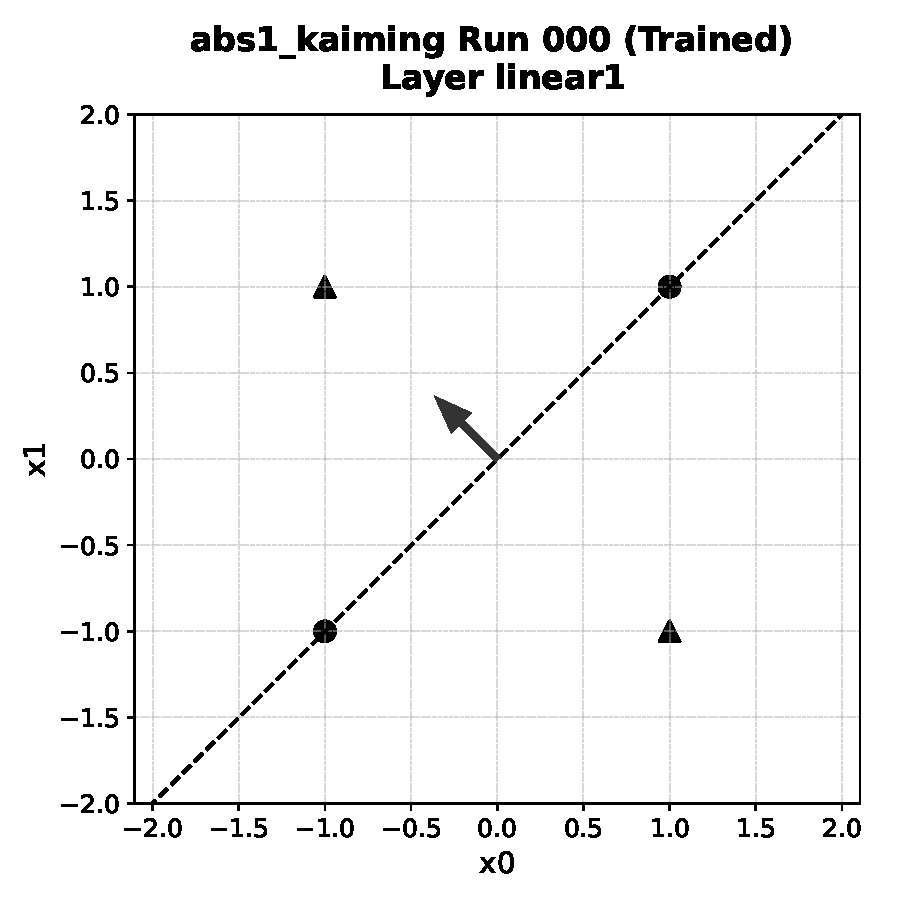
\includegraphics[width=\linewidth]{abs1/figs/kaiming_run000.pdf}
    \caption{Run 000}
  \end{subfigure}\hfill
  \begin{subfigure}{0.46\textwidth}
    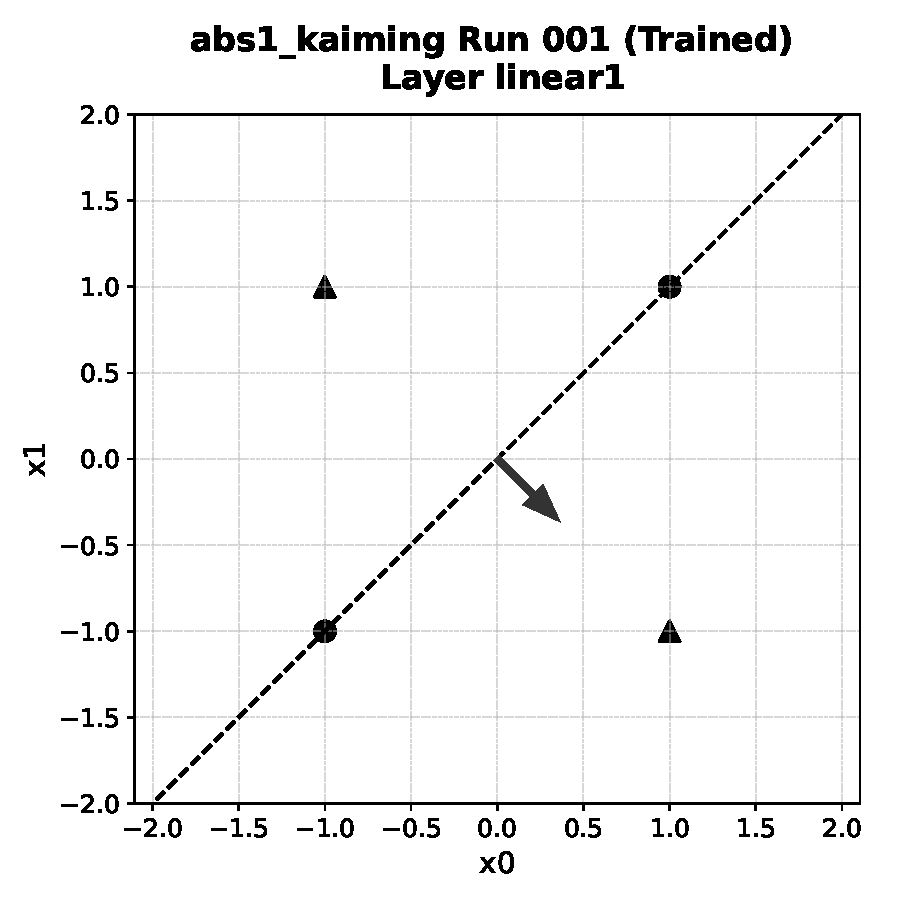
\includegraphics[width=\linewidth]{abs1/figs/kaiming_run001.pdf}
    \caption{Run 001 (sign-flip)}
  \end{subfigure}
  \caption{Two mirror-symmetric prototype surfaces learned under the
           \textsc{Kaiming} initializer.  
           Dashed line: \(f(x)=0\).  
           \(\bullet\): class-False points (output = 0).  
           \(\blacktriangle\): class-True points (output = 1).}
  \label{fig:abs1-hyperplanes}
\end{figure}

\paragraph{Interpretation.}
\begin{itemize}
  \item \textbf{Distance clusters.}  
        All five initializers collapse to a single distance pattern:
        the False points lie \emph{exactly} on the surface
        ($d_{\text{False}}=0$) and the True points lie \(\sqrt2\) away.
        This confirms that the neuron represents class identity via the
        \emph{location} of its zero-level set rather than by large positive
        activations.
  \item \textbf{Weight clusters.}  
        DBSCAN ($eps = 0.1$, $min_samples = 2$) always discovers two parameter clusters whose centroids are
        sign flips of one another,
        \((\frac12,-\frac12,0)\) and \((-\frac12,\frac12,0)\).
        Figure~\ref{fig:abs1-hyperplanes} visualises the corresponding
        hyperplanes for two \textsc{Kaiming} runs, illustrating the
        mirror-image symmetry that stems from the centred XOR data.
\end{itemize}

\paragraph{Why this matters for Prototype-Surface Learning.}
Prototype-Surface Learning argues that a neuron’s meaning is anchored by
where its pre-activation is zero.  The empirical geometry here shows exactly
that behaviour: training \emph{locks} the surface onto the negative prototypes
and positions the positive prototypes on parallel offsets.  Because those
parallel offsets never cross zero, they are implicit but fully determined once
the prototype surface is in place.

Together with the convergence results, the geometry demonstrates that weight
scale affects only the optimisation \emph{speed}; the final surface—and
therefore the learned representation—remains invariant across all
initialization schemes.

% ------------------------------------------------------------------
\subsection*{Conclusion}

Weight scale sets the pace; geometry remains invariant.  Tiny and Normal
inits converge fastest because they start near the optimal norm; Large
requires the optimiser to shrink weights by an order of magnitude before fine
tuning.  Yet all initializers reach the same two mirror solutions, achieve
$100\,\%$ accuracy, and reproduce the analytically optimal prototype surface.
Future chapters will test whether this separation of \emph{speed} (scale) and
\emph{destination} (geometry) generalises to deeper networks and more complex
datasets.


